%%%%%%%%%%%%%%%%%%%%%%%%%%%%%%%%%%%%%%%%%
% Programming/Coding Assignment
% LaTeX Template
%
% This template has been downloaded from:
% http://www.latextemplates.com
%
% Original author:
% Ted Pavlic (http://www.tedpavlic.com)
%
% Note:
% The \lipsum[#] commands throughout this template generate dummy text
% to fill the template out. These commands should all be removed when 
% writing assignment content.
%
% This template uses a Perl script as an example snippet of code, most other
% languages are also usable. Configure them in the "CODE INCLUSION 
% CONFIGURATION" section.
%
%%%%%%%%%%%%%%%%%%%%%%%%%%%%%%%%%%%%%%%%%

%%%%%%%%%%%%%%%%%%%%%%%%%%%%%%%%%%%%%%%%%%%%%%
% Modified by George Z. Zachos
% on March 28, 2017 for the Parallel Systems
% and Programming course @cse.uoi.gr
%%%%%%%%%%%%%%%%%%%%%%%%%%%%%%%%%%%%%%%%%%%%%%

%----------------------------------------------------------------------------------------
%	PACKAGES AND OTHER DOCUMENT CONFIGURATIONS
%----------------------------------------------------------------------------------------

\documentclass{article}

\usepackage{fancyhdr} % Required for custom headers
\usepackage{lastpage} % Required to determine the last page for the footer
\usepackage{extramarks} % Required for headers and footers
\usepackage[usenames,dvipsnames]{xcolor} % Required for custom colors
\usepackage{graphicx} % Required to insert images
\usepackage{listings} % Required for insertion of code
\usepackage{courier} % Required for the courier font

% Margins
\topmargin=-0.45in
\evensidemargin=0in
\oddsidemargin=0in
\textwidth=6.5in
\textheight=9.0in
\headsep=0.25in

\linespread{1.1} % Line spacing

% Set up the header and footer
\pagestyle{fancy}
\lhead{\hmwkAuthorName} % Top left header
\chead{\hmwkClass: \hmwkTitle} % Top center head
\rhead{\firstxmark} % Top right header
\lfoot{\lastxmark} % Bottom left footer
\cfoot{} % Bottom center footer
\rfoot{Page\ \thepage\ of\ \protect\pageref{LastPage}} % Bottom right footer
\renewcommand\headrulewidth{0.4pt} % Size of the header rule
\renewcommand\footrulewidth{0.4pt} % Size of the footer rule

%\setlength\parindent{0pt} % Removes all indentation from paragraphs

%----------------------------------------------------------------------------------------
%	CODE INCLUSION CONFIGURATION
%----------------------------------------------------------------------------------------

\definecolor{MyDarkGreen}{rgb}{0.0,0.4,0.0} % This is the color used for comments
\lstloadlanguages{C}
\lstset{language=C,
%         commentstyle=\color{magenta}\itshape,
        morekeywords={pthread_t, pthread_cond_t, pthread_mutex_t},
%         keywordstyle=\color{blue},
%         emphstyle=\color{red},
        breaklines,
        basicstyle=\ttfamily,
        stringstyle=\color{magenta},
%         identifierstyle=\color{cyan}
        frame=single, % Single frame around code
        basicstyle=\ttfamily, % Use small true type font
        showstringspaces=false, % Don't put marks in string spaces
        tabsize=5, % 5 spaces per tab
%         morecomment=[l][\color{Blue}]{...}, % Line continuation (...) like blue comment
        numbers=left, % Line numbers on left
        firstnumber=0, % Line numbers start with line 0
        numberstyle=\small\color{Blue}, % Line numbers are blue and small
        stepnumber=1 % Line numbers go in steps of 1
}

% Creates a new command to include a perl script, the first parameter is the filename of the script (without .pl), the second parameter is the caption
\newcommand{\cscript}[2]{
\begin{itemize}
\item[]\lstinputlisting[caption=#2,label=#1]{#1.c}
\end{itemize}
}

\def\code#1{\texttt{#1}}
%----------------------------------------------------------------------------------------
%	DOCUMENT STRUCTURE COMMANDS
%	Skip this unless you know what you're doing
%----------------------------------------------------------------------------------------

% Header and footer for when a page split occurs within a problem environment
\newcommand{\enterProblemHeader}[1]{
\nobreak\extramarks{#1}{#1 continued on next page\ldots}\nobreak
\nobreak\extramarks{#1 (continued)}{#1 continued on next page\ldots}\nobreak
}

% Header and footer for when a page split occurs between problem environments
\newcommand{\exitProblemHeader}[1]{
\nobreak\extramarks{#1 (continued)}{#1 continued on next page\ldots}\nobreak
\nobreak\extramarks{#1}{}\nobreak
}

\setcounter{secnumdepth}{0} % Removes default section numbers
\newcounter{homeworkProblemCounter} % Creates a counter to keep track of the number of problems

\newcommand{\homeworkProblemName}{}
\newenvironment{homeworkProblem}[1][Problem \arabic{homeworkProblemCounter}]{ % Makes a new environment called homeworkProblem which takes 1 argument (custom name) but the default is "Problem #"
\stepcounter{homeworkProblemCounter} % Increase counter for number of problems
\renewcommand{\homeworkProblemName}{#1} % Assign \homeworkProblemName the name of the problem
\section{\homeworkProblemName} % Make a section in the document with the custom problem count
\enterProblemHeader{\homeworkProblemName} % Header and footer within the environment
}{
\exitProblemHeader{\homeworkProblemName} % Header and footer after the environment
}

\newcommand{\problemAnswer}[1]{ % Defines the problem answer command with the content as the only argument
\noindent\framebox[\columnwidth][c]{\begin{minipage}{0.98\columnwidth}#1\end{minipage}} % Makes the box around the problem answer and puts the content inside
}

\newcommand{\homeworkSectionName}{}
\newenvironment{homeworkSection}[1]{ % New environment for sections within homework problems, takes 1 argument - the name of the section
\renewcommand{\homeworkSectionName}{#1} % Assign \homeworkSectionName to the name of the section from the environment argument
\subsection{\homeworkSectionName} % Make a subsection with the custom name of the subsection
\enterProblemHeader{\homeworkProblemName\ [\homeworkSectionName]} % Header and footer within the environment
}{
\enterProblemHeader{\homeworkProblemName} % Header and footer after the environment
}

%----------------------------------------------------------------------------------------
%	NAME AND CLASS SECTION
%----------------------------------------------------------------------------------------

\newcommand{\hmwkTitle}{Homework \#1} % Assignment title
\newcommand{\hmwkDueDate}{Monday,\ April\ 3,\ 2017} % Due date
\newcommand{\hmwkClass}{MYE023} % Course/class
\newcommand{\hmwkClassTime}{} % Class/lecture time
\newcommand{\hmwkClassInstructor}{Vassilios V. Dimakopoulos} % Teacher/lecturer
\newcommand{\hmwkAuthorName}{George Z. Zachos} % Your name

%----------------------------------------------------------------------------------------
%	TITLE PAGE
%----------------------------------------------------------------------------------------

\title{
\vspace{2in}
\textmd{\textbf{\hmwkClass:\ \hmwkTitle}}\\
\normalsize\vspace{0.1in}\small{Due\ on\ \hmwkDueDate}\\
\vspace{0.1in}\large{\textit{\hmwkClassInstructor}}
\vspace{3in}
}

\author{\textbf{\hmwkAuthorName}}
\date{April 2, 2017} % Insert date here if you want it to appear below your name

%----------------------------------------------------------------------------------------

\setcounter{secnumdepth}{3}

\begin{document}

\maketitle

%----------------------------------------------------------------------------------------
%	TABLE OF CONTENTS
%----------------------------------------------------------------------------------------

\newpage
\tableofcontents
\newpage


%+----------------------------------------------------------+
%|                                                          |
%|          EXERCISE #1                                     |
%|                                                          |
%+----------------------------------------------------------+

\section{Exercise \#1}

\subsection{About}
This exercise is about the calculation of the mathematical constant $\pi$ using \texttt{POSIX}
threads and dynamic scheduling. During dynamic scheduling the parallelizable loops are divided
into chunks of iterations (tasks) and are dispatched to the threads available to the runtime
system for execution. The dispatch takes place in respect to the current processor workload
where each thread executes and as a result load balancing is achieved. In case chunk size is
one ($1$) iteration, we refer to this technique as self-scheduling. The purpose of this
exercise is to time the calculation of $\pi$ and observe how altering the number of threads
will affect execution time for a given chunk size.

\subsection{Experiment details}
The calculation consists of $5*10^8$ loop iterations, while thread number takes value in \{1, 4, 16\} and
chunk size in \{1, 10, $10^2$, $10^3$, $10^4$, $10^5$\}.

\subsubsection{System Specifications}
The experiments were conducted on a Dell OptiPlex 7020:
\begin{itemize}
 \item CPU: Intel\textregistered \ Core\texttrademark \ i5-4590 CPU @ 3.30GHz (64 bit)
 \item RAM: 2 DIMMs x4GiB @ 1600MHz DDR3
 \item Cache line size: 64B (in all levels)
 \item Cache associativity:
 \begin{itemize}
  \item L1, L2: 8-way set associative
  \item L3: 12-way set associative
 \end{itemize}
\end{itemize}

\begin{figure}[htbp]
  \centering
  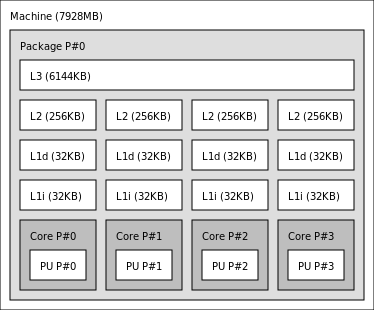
\includegraphics[width=0.5\columnwidth]{./opti7020-topo.png}
  \caption{Topology information of a Dell OptiPlex 7020}
\end{figure}

\pagebreak

\subsection{Timing Results}
In the following tables and plots the recorded execution times are displayed.
Note that $X$ axis is plotted on a (base 2) \underline{logarithmic} scale while
$Y$ axis on a \underline{linear} scale.

%------------------------------------ 1

\begin{table}[htbp]
  \centering
    \begin{tabular}{|c c||l l l l| l|} 
    \hline
    \multicolumn{7}{|c|}{Timing results of $\pi$ calculation (Time unit: seconds)} \\
    \hline
    Chunk Size & \# of threads & 1st run & 2nd run & 3rd run & 4th run & Average time\\ [0.5ex] 
    \hline\hline
    1 & 1 & 18.451202 & 18.443870 & 18.444319 & 18.441278 & 18.44516725 \\ 
    \hline
    1 & 4 & 98.559317 & 98.393137 & 99.515415 & 98.189223 & 98.664273 \\
    \hline
    1 & 16 & 95.482310 & 95.205719 & 95.275233 & 95.197046 & 95.290077 \\ [1ex]
    \hline
    \end{tabular}
  \caption{Timing results of $\pi$ calculation using chunk size = 1 iteration}
\end{table}


\begin{figure}[htbp]
  \centering
  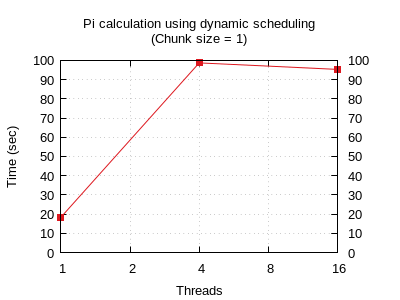
\includegraphics[width=0.55\columnwidth]{../ex1/plots/pi_c1.png}
  \caption{Timing results of $\pi$ calculation using chunk size = 1 iteration}
\end{figure}

%------------------------------------ 2

\begin{table}[htbp]
  \centering
    \begin{tabular}{|c c||l l l l| l|} 
    \hline
    \multicolumn{7}{|c|}{Timing results of $\pi$ calculation (Time unit: seconds)} \\
    \hline
    Chunk Size & \# of threads & 1st run & 2nd run & 3rd run & 4th run & Average time\\ [0.5ex] 
    \hline\hline
    10 & 1 & 6.505206 & 6.510850 & 6.507051 & 6.511070 & 6.50854425 \\
    \hline
    10 & 4 & 10.843631 & 10.728116 & 10.715714 & 10.832101 & 10.7798905 \\
    \hline
    10 & 16 & 10.829372 & 10.820372 & 10.842818 & 10.748566 & 10.810282 \\ [1ex]
    \hline
    \end{tabular}
  \caption{Timing results of $\pi$ calculation using chunk size = 10 iteration}
\end{table}

\begin{figure}[htbp]
  \centering
  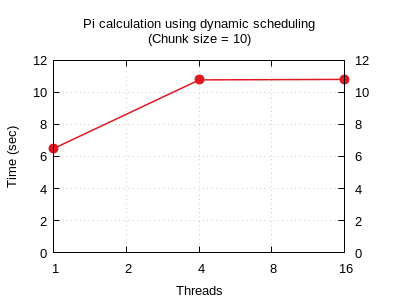
\includegraphics[width=0.55\columnwidth]{../ex1/plots/pi_c10.png}
  \caption{Timing results of $\pi$ calculation using chunk size = 10 iterations}
\end{figure}

%------------------------------------ 3

\begin{table}[htbp]
  \centering
    \begin{tabular}{|c c||l l l l| l|} 
    \hline
    \multicolumn{7}{|c|}{Timing results of $\pi$ calculation (Time unit: seconds)} \\
    \hline
    Chunk Size & \# of threads & 1st run & 2nd run & 3rd run & 4th run & Average time\\ [0.5ex] 
    \hline\hline
    100 & 1 & 6.275921 & 6.279012 & 7.893470 & 6.281098 & 6.68237525 \\
    \hline
    100 & 4 & 2.428611 & 2.464799 & 2.463414 & 2.425332 & 2.445539 \\
    \hline
    100 & 16 & 2.425184 & 2.459710 & 2.432488 & 2.458897 & 2.44406975 \\ [1ex]
    \hline
    \end{tabular}
  \caption{Timing results of $\pi$ calculation using chunk size = 100 iteration}
\end{table}

\begin{figure}[htbp]
  \centering
  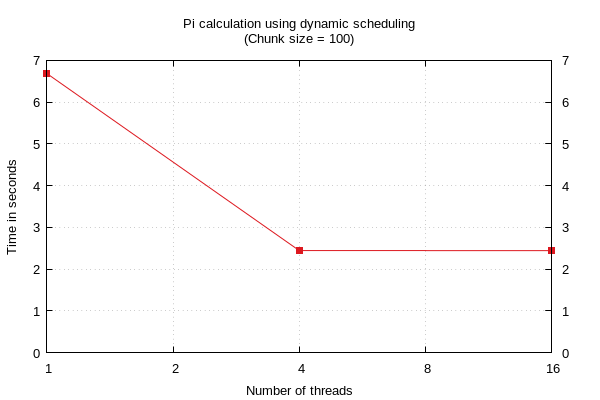
\includegraphics[width=0.55\columnwidth]{../ex1/plots/pi_c100.png}
  \caption{Timing results of $\pi$ calculation using chunk size = 100 iterations}
\end{figure}

%------------------------------------ 4

\begin{table}[htbp]
  \centering
    \begin{tabular}{|c c||l l l l| l|} 
    \hline
    \multicolumn{7}{|c|}{Timing results of $\pi$ calculation (Time unit: seconds)} \\
    \hline
    Chunk Size & \# of threads & 1st run & 2nd run & 3rd run & 4th run & Average time\\ [0.5ex] 
    \hline\hline
    1000 & 1 & 6.248489 & 6.254362 & 6.254913 & 6.251492 & 6.252314 \\
    \hline
    1000 & 4 & 1.733363 & 1.735331 & 1.732440 & 1.734742 & 1.733969 \\
    \hline
    1000 & 16 & 1.731060 & 1.726669 & 1.730891 & 1.732937 & 1.73038925 \\ [1ex]
    \hline
    \end{tabular}
  \caption{Timing results of $\pi$ calculation using chunk size = 1000 iteration}
\end{table}

\begin{figure}[htbp]
  \centering
  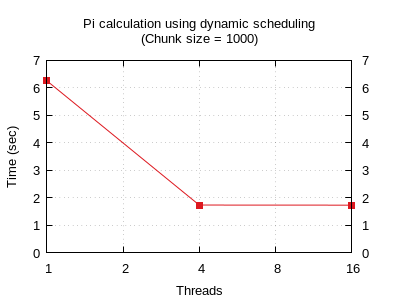
\includegraphics[width=0.55\columnwidth]{../ex1/plots/pi_c1000.png}
  \caption{Timing results of $\pi$ calculation using chunk size = 1000 iterations}
\end{figure}

%------------------------------------ 5


\begin{table}[htbp]
  \centering
    \begin{tabular}{|c c||l l l l| l|} 
    \hline
    \multicolumn{7}{|c|}{Timing results of $\pi$ calculation (Time unit: seconds)} \\
    \hline
    Chunk Size & \# of threads & 1st run & 2nd run & 3rd run & 4th run & Average time\\ [0.5ex] 
    \hline\hline
    10000 & 1 & 6.244337 & 6.252478 & 6.250002 & 6.252064 & 6.24972025 \\
    \hline
    10000 & 4 & 1.664214 & 1.659239 & 1.660260 & 1.659163 & 1.660719 \\
    \hline
    10000 & 16 & 1.660762 & 1.664066 & 1.661164 & 1.658869 & 1.66121525 \\ [1ex]
    \hline
    \end{tabular}
  \caption{Timing results of $\pi$ calculation using chunk size = 10000 iteration}
\end{table}

\begin{figure}[htbp]
  \centering
  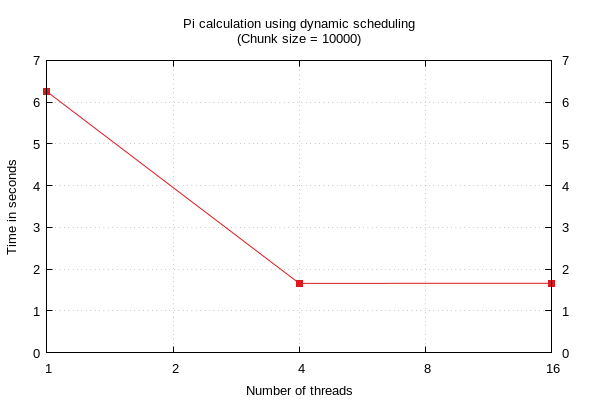
\includegraphics[width=0.55\columnwidth]{../ex1/plots/pi_c10000.png}
  \caption{Timing results of $\pi$ calculation using chunk size = 10000 iterations}
\end{figure}

%------------------------------------ 6


\begin{table}[htbp]
  \centering
    \begin{tabular}{|c c||l l l l| l|} 
    \hline
    \multicolumn{7}{|c|}{Timing results of $\pi$ calculation (Time unit: seconds)} \\
    \hline
    Chunk Size & \# of threads & 1st run & 2nd run & 3rd run & 4th run & Average time\\ [0.5ex] 
    \hline\hline
    100000 & 1 & 6.237799 & 6.234975 & 6.244593 & 6.235083 & 6.2381125 \\
    \hline
    100000 & 4 & 1.661888 & 1.658459 & 1.667569 & 1.651900 & 1.659954 \\
    \hline
    100000 & 16 & 1.653965 & 1.652250 & 1.651300 & 1.651015 & 1.6521325 \\ [1ex]
    \hline
    \end{tabular}
  \caption{Timing results of $\pi$ calculation using chunk size = 100000 iteration}
\end{table}

\begin{figure}[htbp]
  \centering
  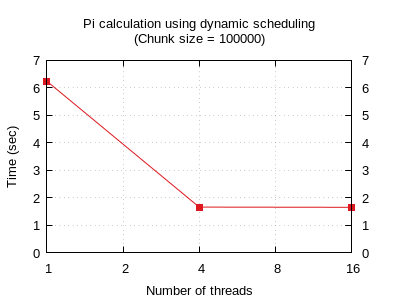
\includegraphics[width=0.55\columnwidth]{../ex1/plots/pi_c100000.png}
  \caption{Timing results of $\pi$ calculation using chunk size = 100000 iterations}
\end{figure}

%------------------------------------
\pagebreak

\subsection{Conclusion}
Based on the results presented above and given that the average execution time of the serial
program is 6,245896 seconds, we conclude that:

\begin{itemize}
 \item Program performance is increased until oversubscription appears. Even though we expect
       overheads to be introduced due to time slicing (e.g. context switching, cache pollution),
       the execution time becomes approximately constant after the number of threads exceeds
       the number of the processors available (4). This happens because switching between
       threads is less resource-intensive than switching between processes.
 \item Self-scheduling leads to execution times multiple times greater than the one of the
       serial program and in case of multithreaded calculation, dozens of times greater.
       The chunk size of one (1) iteration is a fine-grained task something that results
       in threads constantly racing to acquire the same mutex lock. As the number of threads
       is increased, race overhead is increased too. Moreover, the granularity of self-scheduling
       leads to more function calls taking place, something that adds up to the existing overheads.
 \item A single thread executing tasks with chunk size $\geq$ 10 requires almost the same time
       as the serial program.
 \item Multiple threads and tasks with chunk size $\ll 10^2$ result in higher execution times
       compared to the serial program. The reasons for these overheads are the same as in
       self-scheduling (fine-grained parallelism).
 \item Parallel program efficiency is unfolded for chunk size $\geq 10^2$ but hits a bottleneck
       for more coarse-grained tasks (chunk size $\geq 10^4$ iterations in this case).
\end{itemize}


%+----------------------------------------------------------+
%|                                                          |
%|          EXERCISE #2                                     |
%|                                                          |
%+----------------------------------------------------------+

\section{Exercise \#2}

\subsection{About}
This exercise is about the multiplication of integer $N$x$N$ arrays using \texttt{POSIX} threads
and static scheduling. During static scheduling the parallelizable loops are evenly (when
possible) divided into chunks of iterations (tasks) and are dispatched to the threads available
to the runtime system for execution. Due to this even distribution of iterations and in contrast
to dynamic scheduling, a thread executing on a processor under heavy workload will increase the
total execution time. The purpose of this exercise is to parallelize only the \underline{outermost}
for-loop of the serial calculation, time the matrix multiplication and observe how altering the
number of threads will affect execution time.

\subsection{Implementation details}
If $T$ is the number of threads, and $N$ is the array dimension, then the outermost
for-loop of the serial program consists of $N$ iterations, that should be divided
into $T$ chunks. When $T$ divides $N$ evenly, the exact chunk size is $N/T$. In the
opposite case, $S=N \bmod T$ threads will be assigned $\lfloor{N/T}\rfloor+1$ iterations
and $T-S$ threads will be assigned $\lfloor{N/T}\rfloor$ iterations. We are going
to refer to $S$ as the number of special threads because these threads execute one
more iteration than the rest. This policy manages to avoid a lopsided distribution
of iterations to threads as it increases workload by only a single iteration
\footnote{This additional iteration may add significant delays in coarse-grained
tasks}.

\newpage

\subsection{Experiment details}
During this experiment, thread number takes value in \{1, 2, 4, 8, 12, 16\} and array
size is 1024x1024.

\subsubsection{System Specifications}
The experiments were conducted once again on a Dell OptiPlex 7020.


\subsection{Timing Results}
In the following table and plot the recorded execution times are displayed.
Note that $X$ axis is plotted on a (base 2) \underline{logarithmic} scale while
$Y$ axis on a \underline{linear} scale.

%------------------------------------ 1

\begin{table}[htbp]
  \centering
    \begin{tabular}{|c||l|l|l|l||l|} 
    \hline
    \multicolumn{6}{|c|}{Timing results of matrix multiplication (Time unit: seconds)} \\
    \multicolumn{6}{|c|}{Array size: 1024x1024} \\
    \hline
   \# of threads & 1st run & 2nd run & 3rd run & 4th run & Average time\\ [0.5ex] 
    \hline\hline
    1 & 5.057095 & 4.319662 & 3.157559 & 5.297035 & 4.45783775 \\ 
    \hline
    2 & 2.648351 & 2.545161 & 1.940197 & 2.043663 & 2.294343 \\
    \hline
    4 & 0.918773 & 0.800195 & 1.504583 & 1.504583 & 1.07884625 \\
    \hline
    8 & 0.971947 & 1.428921 & 1.224236 & 0.990774 & 1.1539695 \\
    \hline
    12 & 0.965793 & 0.986273 & 0.981548 & 1.130868 & 1.0161205 \\
    \hline
    16 & 1.208460 & 1.241845 & 1.015431 & 0.974093 & 1.10995725 \\ [1ex]
    \hline
    \end{tabular}
  \caption{Timing results of 2D matrix multiplication}
\end{table}


\begin{figure}[htbp]
  \centering
  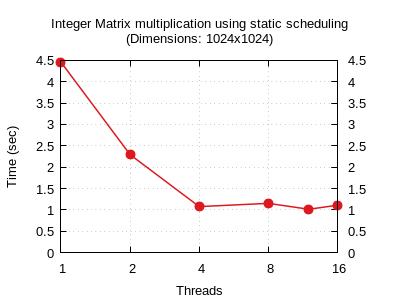
\includegraphics[width=0.55\columnwidth]{../ex2/plots/matmul.png}
  \caption{Timing results of 2D matrix multiplication}
\end{figure}

%------------------------------------
\pagebreak

\subsection{Conclusion}
Based on the results presented above and given that the average execution time of the serial
program is 4,297561 seconds, we conclude that:

\begin{itemize}
 \item Program performance is approximately doubled as the number of threads is increased, until
       oversubscription bottleneck is hit and execution time becomes almost constant
       \footnote{This is also the conclusion we came to on Exercise \#1}.
 \item Execution time of the parallel program when a single thread is used to perform the
       calculation is a bit higher than the time of the serial program. Moreover, we observed
       that execution time in general varies from time to time. Several reasons such as context
       switching, thread affinity, cache misses \& cache pollution justify the existence of
       these overheads and consequently this behavior.
\end{itemize}

%+----------------------------------------------------------+
%|                                                          |
%|          EXERCISE #3                                     |
%|                                                          |
%+----------------------------------------------------------+

\section{Exercise \#3}

\subsection{About}
This exercise is about implementing a (simple) custom barrier for a group of \texttt{POSIX}
threads using only integer data types and \texttt{POSIX} condition variables \footnote{The 
use of global variables is not allowed}. The purpose of this exercise is to observe how
altering the number of threads will affect execution time of user programs and how it is
compared to the execution time while using the \texttt{POSIX} threads' barrier implementation.


\subsection{Experiment details}
During this experiment, thread number takes value in \{1, 2, 4, 8, 32, 128, 512, 1024\}.

\subsubsection{System Specifications}
The experiments were conducted once again on a Dell OptiPlex 7020.

\subsection{Implementation Details}
Implementing the barrier synchronization mechanism required definition of struct
\code{barrier\_s} and of the following three functions:

\begin{verbatim}
 int barrier_init(barrier_t *barrier, unsigned int nthr);
 int barrier_wait(barrier_t *barrier);
 int barrier_destroy(barrier_t *barrier);
\end{verbatim}

\cscript{code/barrier_s}{Struct \code{barrier\_s}}

\subsubsection{Struct \code{barrier\_s}}
Struct \code{barrier\_s} contains all the info required to implement the custom barrier and
consists of the following members:
\begin{itemize}
  \item \code{init\_count} : unsigned int \\
        The number of threads that must call \code{barrier\_wait()} before any of them
        return to the caller.
  \item \code{arrived} : unsigned int \\
        The number of threads that have arrived to the barrier; Have called \code{barrier\_wait()}
        and are currently blocked.
  \item \code{left} : unsigned int \\
        The number of threads that have left the barrier; Returned from the \code{barrier\_wait()}
        call.
  \item \code{release\_threads} : pthread\_cond\_t \\
        The threads arriving at the barrier block on this condition variable until all
        \code{init\_count} threads arrive.
  \item \code{next\_bar} : pthread\_cond\_t \\
        The threads arriving at the barrier, while threads from a previous phase are currently
        leaving the barrier, block on this condition variable until all \code{init\_count}
        threads have left and the barrier can be reused.
\end{itemize}

\subsubsection{\code{barrier\_init()}}
The \code{barrier\_init()} function allocates the resources required to use the barrier
referenced by \underline{barrier} and initializes them as needed. The implementation of
this function is pretty straightforward so I am not going to further explain how it works.
The results are undefined if this function is called when any thread is blocked on the
barrier or \underline{barrier} is not initilized. If \code{barrier\_init()} function fails,
the contents of the barrier are undefined. Upon successful completion, this function returns
zero unless one of the following errors occurs:
\begin{itemize}
 \item \code{EINVAL}: The value specified by \underline{count} is equal to zero or
       \underline{barrier} is \code{NULL}.
 \item \code{ENOMEM}: Insufficient memory exists to initialize the barrier.
 \item \code{EBUSY}: If the implementation detects that the \underline{barrier} argument
       refers to an already initialized barrier object.
\end{itemize}

\subsubsection{\code{barrier\_destroy()}}
The \code{barrier\_destroy()} function destroys the barrier referenced by \underline{barrier}
and releases the resources it currently holds. The implementation of this function is pretty
straightforward too so I am not going to further explain how it works. Use of the \underline{barrier}
after calling \code{barrier\_destroy()} is undefined. The results are undefined if this function is
called when any thread is blocked on the barrier or \underline{barrier} is not initilized.
Upon successful completion, this function returns zero unless the following error occurs:
\begin{itemize}
 \item \code{EINVAL}: The barrier object referenced by \underline{barrier} is \code{NULL}.
\end{itemize}

\subsubsection{\code{barrier\_wait()}}
The \code{barrier\_wait()} function synchronizes participating threads at the barrier referenced
by \underline{barrier}. The calling thread blocks until \code{init\_count}\footnote{Has the same
value as \code{count}, specified during \code{barrier\_init()} call.} threads have called 
\code{barrier\_wait()} specifying the very same barrier object. When the required number of
threads have arrived at the barrier, all threads are unblocked and the \underline{barrier}
is reset for future usage. The results are undefined if this function is called with an
uninitialized barrier. Upon successful completion, this function returns
\code{PTHREAD\_BARRIER\_SERIAL\_THREAD} \footnote{Constant defined in \code{pthread.h}}
to a single arbitrary thread synchronized to the barrier and zero to the remaining threads
synchronized. Function \code{barrier\_wait()} may fail with the following error:
\begin{itemize}
 \item \code{EINVAL}: The barrier object referenced by \underline{barrier} is \code{NULL}.
\end{itemize}

\hspace{-0.6cm} The \code{barrier\_wait(barrier\_t *barrier)} function works as follows:
\begin{enumerate}
 \item If \underline{barrier} argument is \code{NULL}, \code{EINVAL} is returned.
 \item The barrier's mutex is locked to ensure that the encountering thread is the only thread around.
 \item In case there are threads exiting the barrier, the encountering thread blocks on barrier's
       condition variable \code{next\_bar}. As soon as it unblocks, it has the mutex lock already
       acquired and proceeds to step \#4 as if this step didn't exist.
 \item The value of member \code{arrived} is incremented.
 \item In case not all \code{init\_count} threads have blocked (arrived) on the barrier, the
       encountering thread blocks on barrier's condition variable \code{release\_threads}.
       As soon as it unblocks, it has the mutex lock acquired and proceeds to step \#6.
 \item The first thread that will reach this part of the code is the last thread that
       called \code{barrier\_wait()}. This happens because only that thead will not block
       on condition variable \code{release\_threads} and will later signal the rest
       \code{init\_count}$-1$ threads.
 \item The value of member \code{left} is incremented.
 \item If the encountering thread is the \underline{first} leaving the barrier, it unblocks all
       threads blocked on \\ \code{release\_threads} condition variable and the function's
       return value is set to\\ \code{PTHREAD\_BARRIER\_SERIAL\_THREAD}.
 \item If the encountering thread is the \underline{last} one leaving the barrier, it resets
       \code{left} and \code{arrived} members to zero and unblocks any threads blocked on
       \code{next\_bar} condition variable as the barrier is ready for reuse.
 \item The barrier's private mutex is unlocked.
 \item Zero is returned unless the return value has been set to \code{PTHREAD\_BARRIER\_SERIAL\_THREAD}.
\end{enumerate}

\hspace{-0.6cm} As you may have observed, the above implementation avoids deadlocks.

\subsection{Bugs}
Concurrently calling \code{barrier\_init()} or \code{barrier\_destroy()} has undefined results.
These two functions should be atomically executed using low level synchronization mechanisms.
Perhaps Linux Kernel Futexes \footnote{Fast Userspace muTEX-es}.

\newpage 

\subsection{Timing Results}
In the following table and plot the recorded execution times are displayed.
Note that $X$ axis is plotted on a (base 2) \underline{logarithmic} scale while
$Y$ axis on a (base 10) \underline{logarithmic} scale.

%------------------------------------ 1

\begin{table}[htbp]
  \centering
    \begin{tabular}{|c||l|l|l|l|l|l|l|l|} 
    \hline
    \multicolumn{9}{|c|}{Timing results of program execution (Time unit: miliseconds)} \\
    \hline
    & \multicolumn{8}{|c|}{\# of threads} \\
    \hline
    Barrier Implemetation  & \multicolumn{1}{|c|}{1} & \multicolumn{1}{|c|}{2} & \multicolumn{1}{|c|}{4} &
    \multicolumn{1}{|c|}{8} & \multicolumn{1}{|c|}{32} & \multicolumn{1}{|c|}{128} & \multicolumn{1}{|c|}{512} & 
    \multicolumn{1}{|c|}{1024}\\
    \hline\hline
    Custom & 0.125 & 0.69325 & 1.56775 & 3.952 & 30.27725 & 119.7172 & 431.333 & 950.200 \\
    \hline
    \texttt{POSIX} threads & 0.085 & 1.09525 & 1.84725 & 3.0225 & 16.98425 & 76.451 & 298.4285 & 643.386 \\
    \hline
    \end{tabular}
  \caption{Timing results of program using barrier-related calls}
\end{table}


\begin{figure}[htbp]
  \centering
  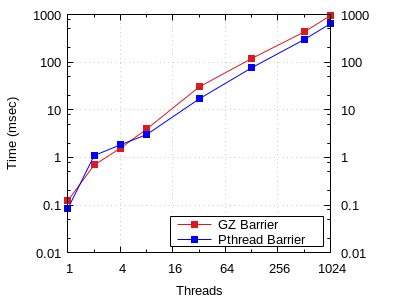
\includegraphics[width=0.55\columnwidth]{../ex3/plots/barrier.png}
  \caption{Timing results of program using barrier-related calls}
\end{figure}

%------------------------------------


\subsection{Conclusion}
Based on the results presented above we conclude that:

\begin{itemize}
 \item User program execution time has a near exponential growth relative to the number of
       threads synchronized by the barrier. This is observed for both the custom and the
       \texttt{POSIX} barrier implementation.
 \item The custom barrier implementation results in higher execution times. This happens
       for the following reasons:
       \begin{enumerate}
         \item The custom barrier implementation is not as optimized as possible because I
         implemented an algorithm I came up with during this assignment.
         \item The custom barrier implementation uses \texttt{POSIX} threads' condition variables
         and a mutex, while the \texttt{POSIX} threads' barrier uses calls to low level synchronization
         mechanisms found in \code{glibc} library\footnote{For more information refer to \code{lowlevellock.h}.}
       \end{enumerate}
\end{itemize}

\end{document}